\documentclass[10pt,twocolumn]{article}
\usepackage[margin=0.75in]{geometry}
\usepackage{graphicx}
\usepackage{booktabs}
\usepackage{amsmath}
\usepackage{hyperref}
\usepackage{enumitem}
\usepackage{xcolor}
\usepackage{caption}

\title{\textbf{Cache Coherence Protocol Simulator:\\Interactive Visualization and Comparative Analysis\\of MSI, MESI, and MOESI Protocols}}
\author{Rushi Patel\\University of California, Riverside\\CS 213 --- Multiprocessor Architecture and Programming}
\date{Spring 2026}

\begin{document}
\maketitle

% ============================================================
\section{Problem Statement and Motivation}
% ============================================================

Cache coherence is a fundamental challenge in shared-memory multiprocessor systems. When multiple processors maintain private caches over a shared address space, a coherence protocol must ensure that all processors observe a consistent view of memory. The three most widely studied snooping-based protocols---MSI, MESI, and MOESI---each make different design tradeoffs between bus traffic, memory writebacks, and implementation complexity.

Despite their importance, these protocols are difficult to reason about from state transition diagrams alone. Students and practitioners must mentally simulate sequences of reads and writes across multiple processors, tracking state changes, bus messages, and data flow simultaneously. This cognitive burden makes it hard to build intuition for \emph{why} one protocol outperforms another in specific access patterns.

This project addresses that gap by building an \textbf{interactive, browser-based cache coherence simulator} that lets users step through memory traces operation-by-operation, observe state transitions in real time, and directly compare MSI, MESI, and MOESI side-by-side with quantitative metrics.

% ============================================================
\section{Background}
% ============================================================

\subsection{Snooping-Based Coherence}

In a snooping protocol, all caches monitor (snoop) a shared bus. When a processor issues a memory operation that misses in its cache or requires exclusive access, it places a bus message (e.g., \texttt{BusRd}, \texttt{BusRdX}, \texttt{BusUpgr}) that other caches observe and react to by updating their local state. Correctness relies on the bus imposing a total order on all transactions, ensuring write serialization---every processor observes writes to the same block in the same order. Combined with the single-writer/multiple-reader (SWMR) invariant, this guarantees coherence.

\subsection{Protocol Overview}

\textbf{MSI} is the baseline protocol with three states: Modified (M), Shared (S), and Invalid (I). Every read miss transitions to S, requiring a \texttt{BusUpgr} on any subsequent write. \textbf{MESI} adds the Exclusive (E) state, which represents a clean, sole copy. A processor that reads a block with no other sharers enters E, allowing a silent upgrade to M on write with zero bus traffic. \textbf{MOESI} further adds the Owned (O) state: when a modified block is read by another processor, the original holder transitions to O (retaining dirty responsibility) instead of writing back to memory, eliminating the writeback entirely.

% ============================================================
\section{Approach and Implementation}
% ============================================================

\subsection{Architecture}

The simulator is implemented as a client-side web application in JavaScript, HTML, and CSS with no build step or server dependency---users simply open \texttt{index.html} in a browser. The architecture follows a clean separation of concerns:

\begin{itemize}[nosep]
  \item \textbf{Protocol layer}: A \texttt{BaseProtocol} class defines the snooping interface. \texttt{MSIProtocol}, \texttt{MESIProtocol}, and \texttt{MOESIProtocol} each implement \texttt{handleCpuRequest()}, encoding the full state machine for that protocol including bus message generation and snoop responses.
  \item \textbf{Simulator core}: The \texttt{Simulator} class manages per-processor caches, shared memory, and a \texttt{Metrics} tracker. It orchestrates each step: applying the requesting processor's transition, broadcasting snoop results to other caches, updating data values, and recording a full snapshot.
  \item \textbf{Trace parser}: Accepts a simple text format (\texttt{P0 R X}, \texttt{P1 W X 5}) with validation, comments, and error reporting.
  \item \textbf{UI layer}: Renders cache state grids, a bus log, step history table, and statistics panel. Supports step-by-step execution, auto-run with adjustable speed, and draggable panel resizing.
\end{itemize}

\subsection{Key Features}

\begin{itemize}[nosep]
  \item \textbf{Single-protocol mode}: Step through a trace viewing per-processor cache states, bus messages, and memory values at each step.
  \item \textbf{Compare mode}: Run the same trace simultaneously on all three protocols, displaying side-by-side cache states and a bar chart of bus traffic, invalidations, and writebacks.
  \item \textbf{Configurable processors}: Support for 2, 3, or 4 processors.
  \item \textbf{Preset traces}: Six traces from course lectures and homework, plus a free-form text input for custom traces.
  \item \textbf{Correctness}: Validated by an automated test suite of 47 tests covering all state transitions, bus messages, snoop behavior, and data value propagation for all three protocols.
\end{itemize}

\begin{figure*}[!bp]
\centering
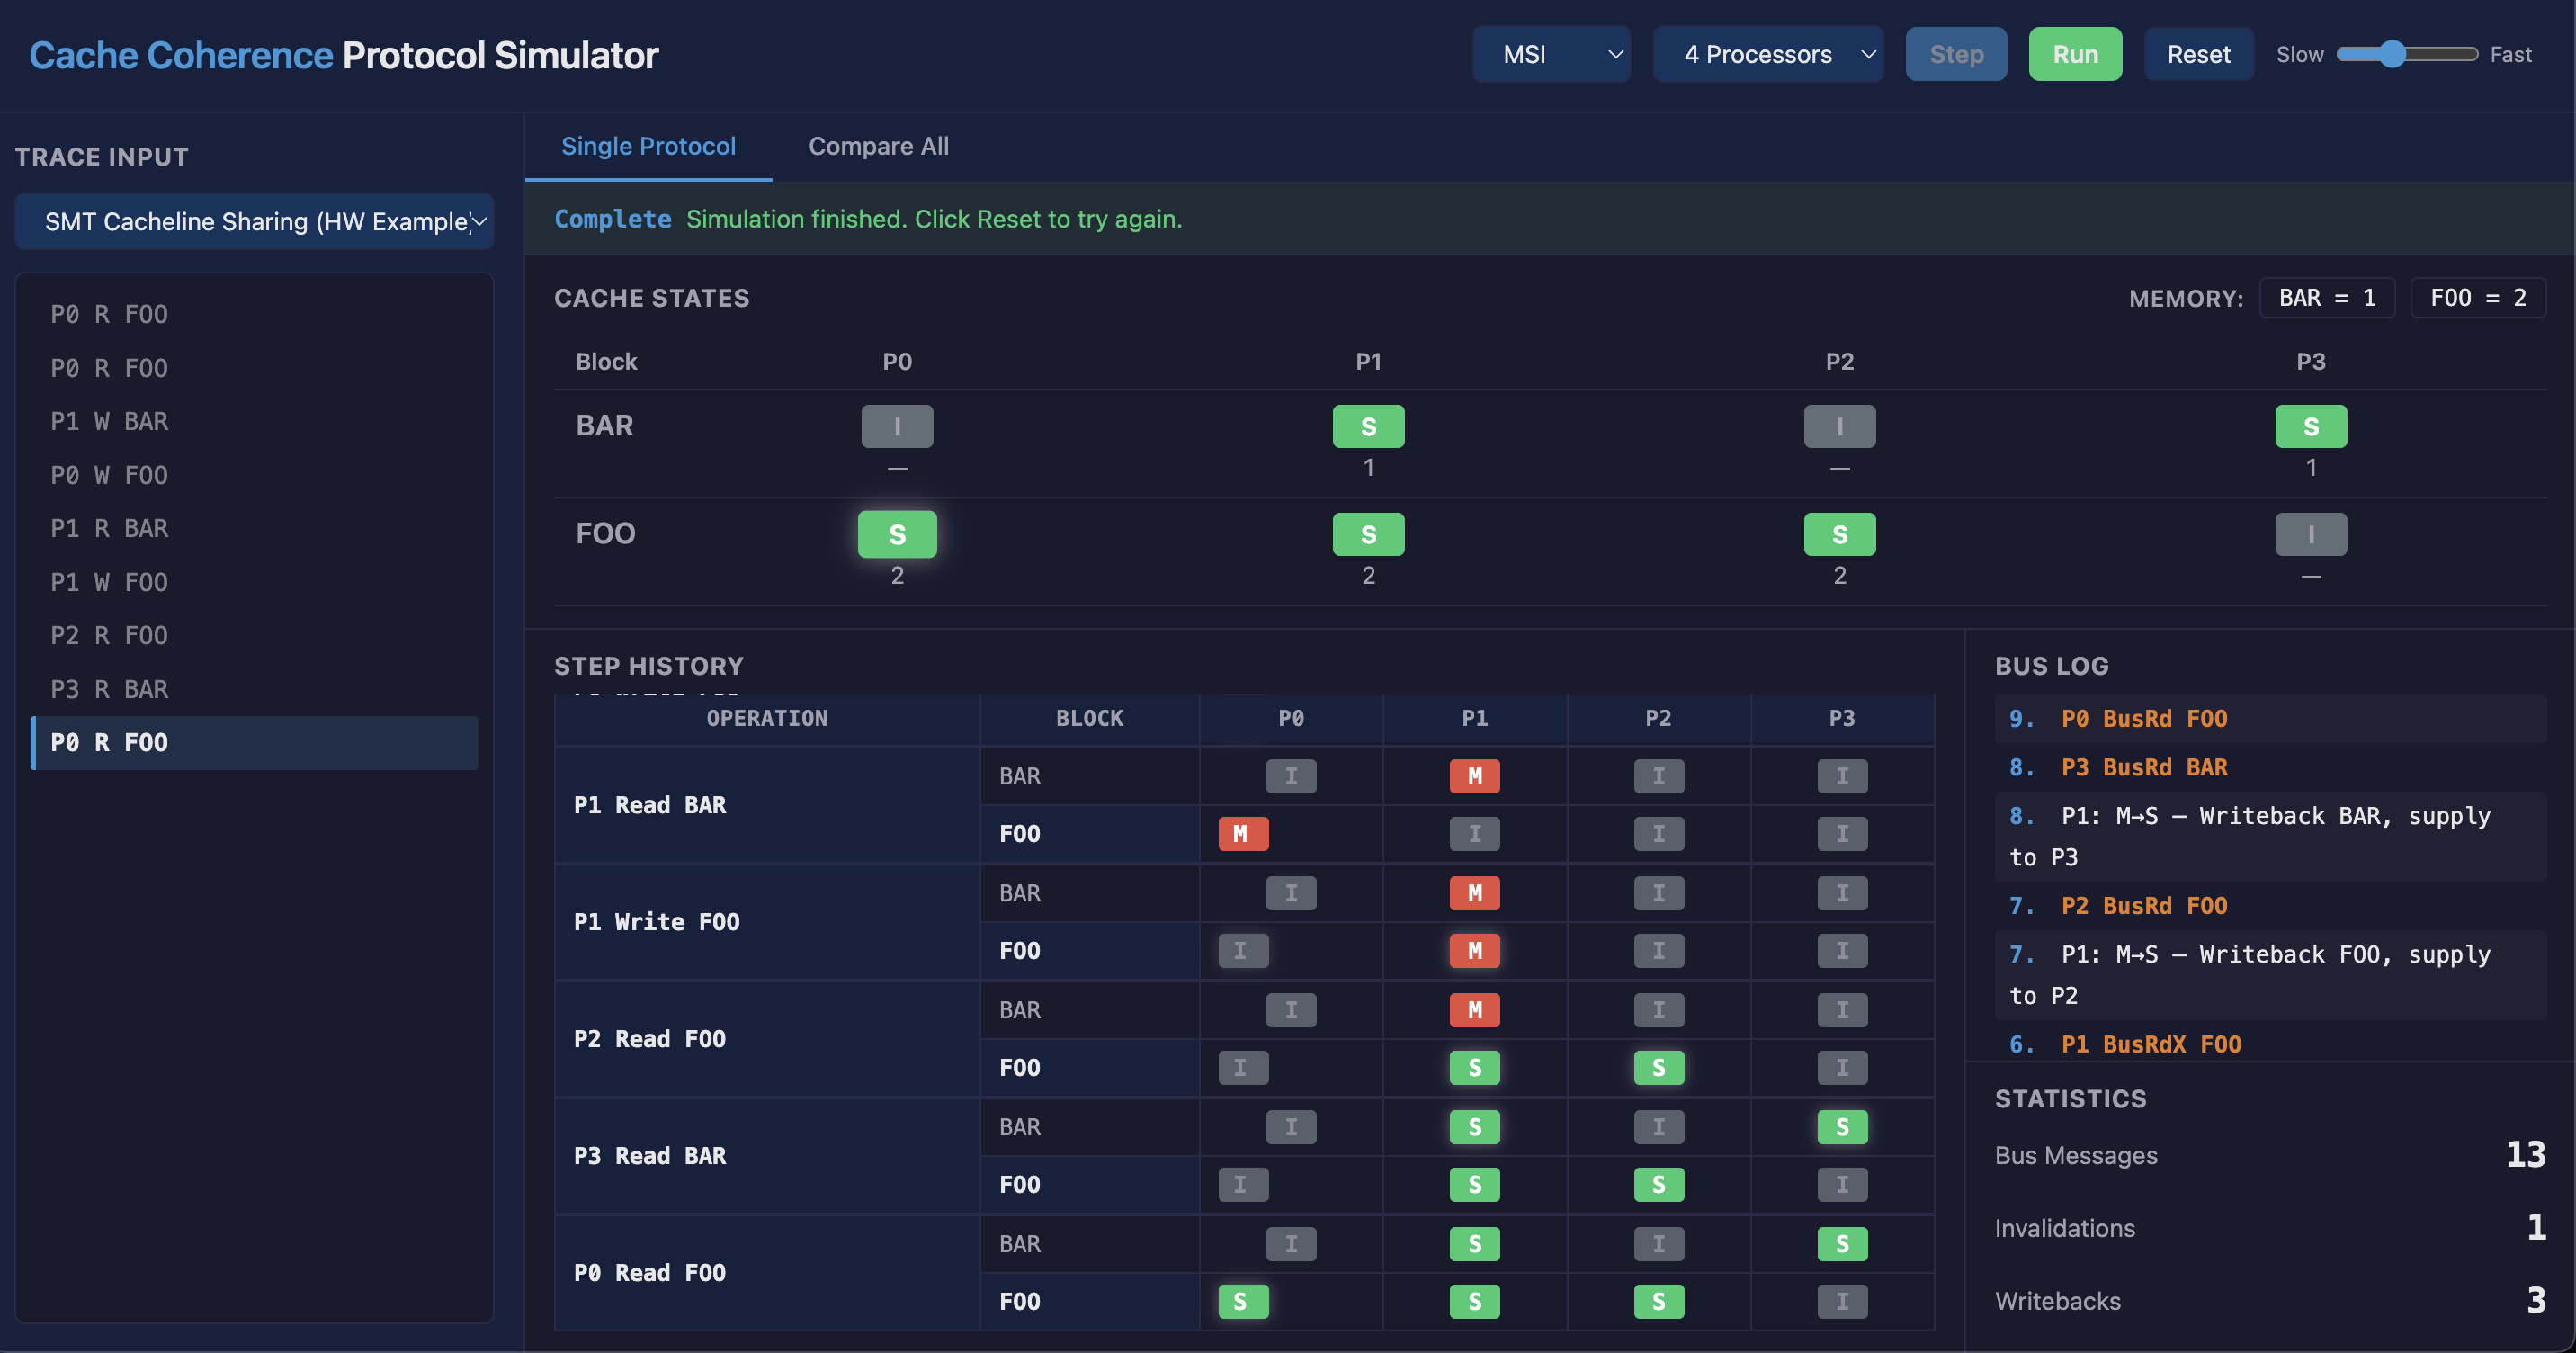
\includegraphics[width=\textwidth]{figures/single-view.png}
\caption{Single-protocol mode showing the SMT Cacheline Sharing trace on MSI with 4 processors. The interface displays cache states (top), step history (bottom-left), bus log and statistics (bottom-right), and memory values (top-right).}
\label{fig:single}
\end{figure*}

% ============================================================
\section{Experimental Methodology}
% ============================================================

To quantitatively compare the three protocols, we designed six trace microbenchmarks, each isolating a specific access pattern that highlights a protocol-level difference (Table~\ref{tab:traces}). These traces are intentionally small to allow step-by-step verification against hand-derived state transitions from lecture, while still being large enough to expose the key behavioral differences between protocols. Each trace was executed on all three protocols using the simulator's core engine. We recorded three metrics:

\begin{itemize}[nosep]
  \item \textbf{Bus traffic}: Total number of bus messages (BusRd, BusRdX, BusUpgr, and flushes).
  \item \textbf{Invalidations}: Number of times a cache line was invalidated due to another processor's write.
  \item \textbf{Writebacks}: Number of dirty-line writebacks to main memory.
\end{itemize}

\begin{table}[h]
\centering
\caption{Trace workloads used for evaluation.}
\label{tab:traces}
\small
\begin{tabular}{@{}lcc@{}}
\toprule
\textbf{Trace} & \textbf{Procs} & \textbf{Ops} \\
\midrule
Basic MSI (Lecture 04) & 2 & 5 \\
MESI Silent Upgrade & 1 & 2 \\
MOESI No Writeback & 2 & 3 \\
3-Proc Contention & 3 & 5 \\
SMT Cacheline Sharing & 4 & 9 \\
Private Data & 3 & 6 \\
\bottomrule
\end{tabular}
\end{table}

% ============================================================
\section{Results and Analysis}
% ============================================================

Figure~\ref{fig:compare} shows the compare mode output for the SMT trace, and Table~\ref{tab:results} presents the full comparison across all traces and protocols.

\begin{figure*}[!bp]
\centering
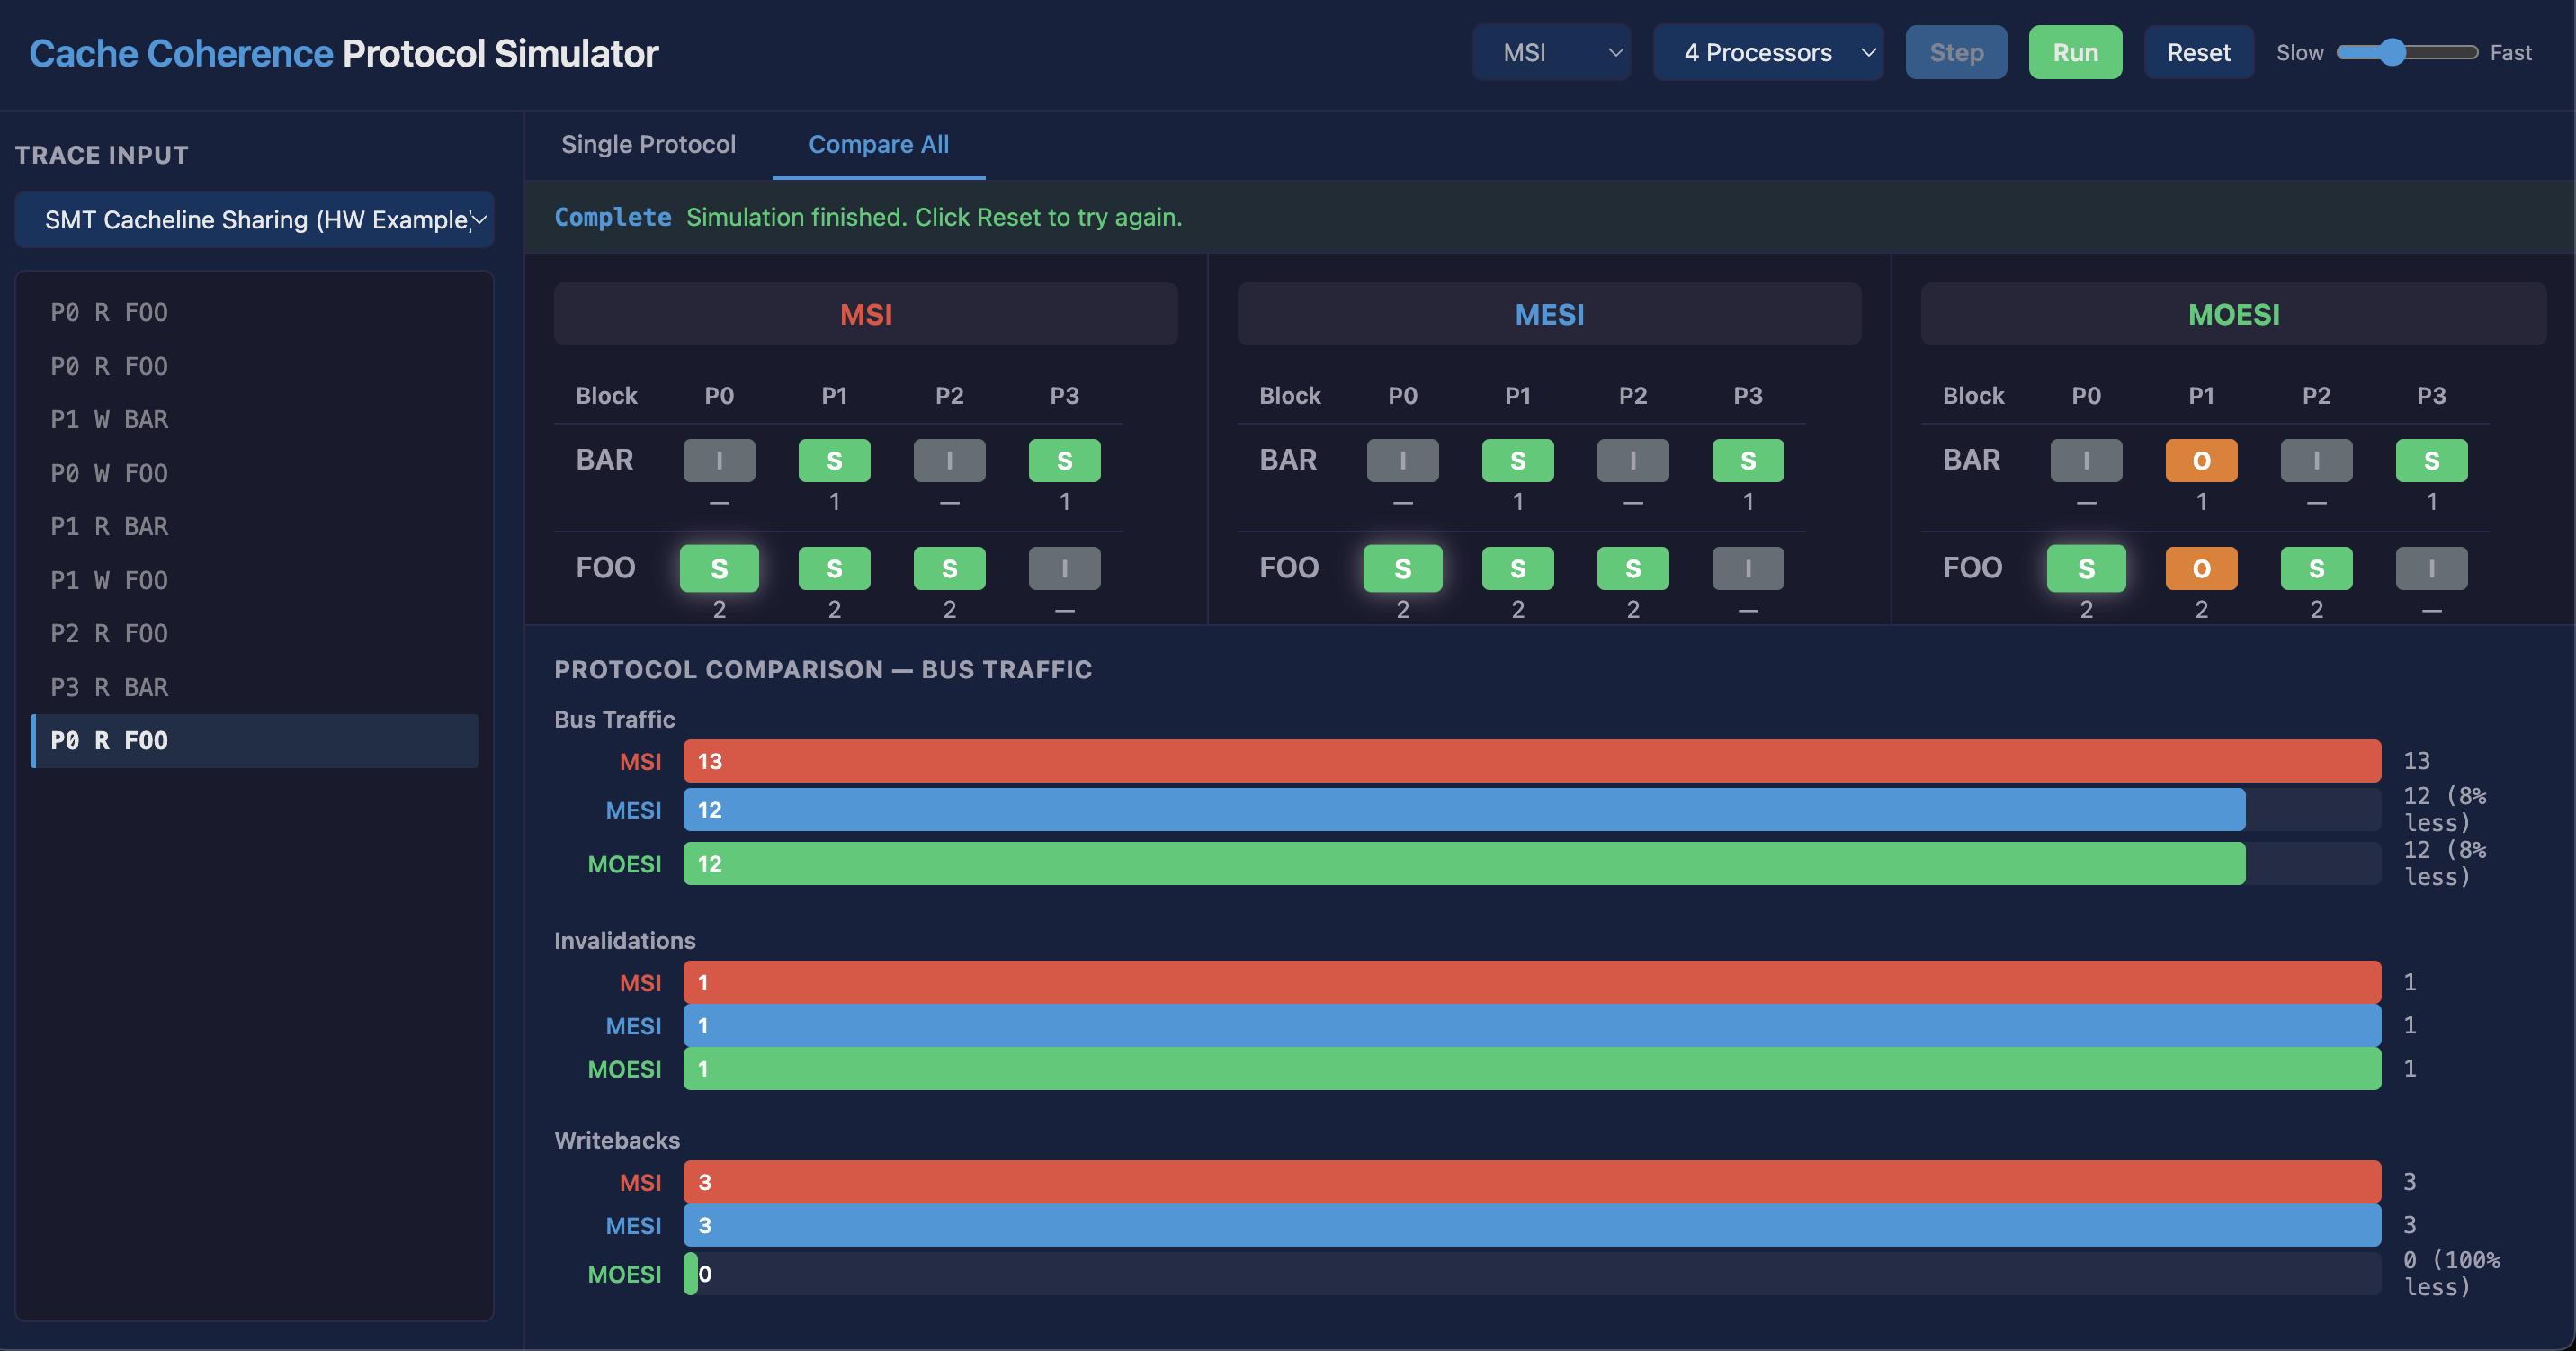
\includegraphics[width=\textwidth]{figures/compare-view.png}
\caption{Compare mode running the SMT Cacheline Sharing trace on all three protocols simultaneously. The bar chart highlights MOESI's elimination of writebacks (0 vs.\ 3, a 100\% reduction) and MESI/MOESI's 8\% bus traffic reduction over MSI.}
\label{fig:compare}
\end{figure*}

\begin{table}[h]
\centering
\caption{Protocol comparison: bus traffic / invalidations / writebacks.}
\label{tab:results}
\small
\begin{tabular}{@{}lccc@{}}
\toprule
\textbf{Trace} & \textbf{MSI} & \textbf{MESI} & \textbf{MOESI} \\
\midrule
Basic MSI        & 8 / 2 / 1 & 8 / 2 / 1 & 8 / 2 / 0 \\
Silent Upgrade   & 3 / 0 / 0 & 2 / 0 / 0 & 2 / 0 / 0 \\
No Writeback     & 5 / 0 / 1 & 4 / 0 / 1 & 4 / 0 / 0 \\
3-Proc Contention & 10 / 4 / 1 & 10 / 4 / 1 & 10 / 4 / 0 \\
SMT Sharing      & 13 / 1 / 3 & 12 / 1 / 3 & 12 / 1 / 0 \\
Private Data     & 9 / 0 / 0 & 6 / 0 / 0 & 6 / 0 / 0 \\
\bottomrule
\end{tabular}
\end{table}

\subsection{MESI Reduces Bus Traffic for Private Data}

The most dramatic difference between MSI and MESI appears in the \emph{Private Data} trace, where each processor reads and writes its own block with no sharing. MSI generates 9 bus messages because every read enters S, requiring a \texttt{BusUpgr} on the subsequent write. MESI detects that the block has no other sharers, places it in E, and silently upgrades to M---\textbf{reducing bus traffic by 33\%} (9 $\to$ 6). The reduction follows directly from the 3 read-write pairs in the trace: each pair saves one \texttt{BusUpgr} in MESI (the E$\to$M upgrade is silent), for a total of 3 fewer messages out of 9. This pattern is common in real workloads where threads operate on thread-local data.

The \emph{Silent Upgrade} trace isolates this mechanism: a single processor reads then writes. MSI needs 3 bus messages (BusRd + BusUpgr + the read response), while MESI needs only 2 (BusRd + response, then silent E$\to$M).

\subsection{MOESI Eliminates Writebacks}

Across \textbf{all six traces}, MOESI produces \textbf{zero writebacks}, compared to MSI and MESI which generate 1--3 writebacks depending on the workload. This is the direct benefit of the Owned state: when a modified block is read by another processor, the holder transitions M$\to$O and supplies data via cache-to-cache transfer, avoiding the memory writeback entirely.

The effect is most pronounced in the \emph{SMT Cacheline Sharing} trace (a 4-core workload with 9 operations), where MSI and MESI produce 3 writebacks while MOESI produces 0---a significant reduction in memory bus bandwidth consumption. We note that this zero-writeback result represents an upper bound: our simulator has unlimited cache capacity and no replacement policy, so eviction-triggered writebacks (O$\to$I with writeback to memory) never occur. In real systems with finite caches, MOESI's writeback savings would be partially offset by eviction traffic under high cache pressure.

\subsection{Invalidation Counts are Protocol-Independent}

Invalidations are identical across all three protocols for every trace. This is expected: invalidations are driven by write operations to shared blocks, and all three protocols must invalidate other sharers on a write. The Exclusive and Owned states optimize \emph{how} data is obtained and \emph{whether} writebacks occur, but they do not change \emph{when} invalidations are necessary.

\subsection{Discussion}

The results confirm the theoretical expectations from the protocol designs:

\begin{enumerate}[nosep]
  \item MESI's E state is a pure optimization for the private-data case, with no downside in shared scenarios (it never performs worse than MSI).
  \item MOESI's O state is a pure optimization for the shared-read-after-write case, eliminating writebacks without increasing bus traffic or invalidations.
  \item The protocols form a strict hierarchy: MSI $\leq$ MESI $\leq$ MOESI in terms of efficiency, which explains why modern processors (e.g., AMD) use MOESI and Intel uses a MESIF variant.
\end{enumerate}

% ============================================================
\section{Conclusion and Lessons Learned}
% ============================================================

We built an interactive cache coherence protocol simulator that visualizes MSI, MESI, and MOESI side-by-side with quantitative metrics. Our experimental comparison across six trace workloads confirms that MESI reduces bus traffic by up to 33\% for private-data patterns through silent E$\to$M upgrades, and MOESI eliminates all memory writebacks through the Owned state's cache-to-cache transfers.

\textbf{Lessons learned:}
\begin{itemize}[nosep]
  \item Implementing the full state machines revealed subtleties not apparent from diagrams alone---particularly around data value propagation (which cache supplies data?) and the interaction between snoop responses and the requesting processor's transition.
  \item The compare mode proved valuable for building intuition: seeing the same trace produce different writeback counts across protocols makes the benefit of each additional state immediately concrete.
  \item A correctness test suite was essential. Several early bugs (e.g., incorrect BusRdX vs.\ BusUpgr selection, missing writeback on M$\to$I transitions) were only caught by systematic testing of all state$\times$operation combinations.
\end{itemize}

\textbf{Limitations and future work:} The simulator models a simplified single-level cache with unlimited capacity and no replacement policy. Extending it with set-associative caches, LRU eviction, and directory-based protocols would bring it closer to real hardware behavior. Adding support for memory consistency models (TSO, relaxed) and fence instructions would further deepen its educational value.

\end{document}
